\documentclass[11pt]{article}
\usepackage[margin=1in]{geometry}
\usepackage[dvipsnames]{xcolor}
\usepackage{booktabs,graphicx,amsmath,hyperref,microtype}
\usepackage[numbers]{natbib}
\hypersetup{colorlinks,linkcolor=blue!50!black,citecolor=blue!50!black,urlcolor=blue!50!black}

\title{Does a hill-climbing skill make coding agents better optimizers?\\[2pt]
\large A controlled benchmark of process instructions, and a check of blind LLM judges against real A/B tests}
\author{Abhay Mettu\\\small\url{https://github.com/abhaymettu/hill-climb}}
\date{November 2026}

\begin{document}
\maketitle

\begin{abstract}
Coding agents are now asked to optimize things over many rounds: make code faster, raise a score, tune a
config. Recipes for doing this (edit, measure, keep or revert) circulate as prompts and agent skills, but none
reports a controlled test of whether the recipe helps. We wrote one such skill, hill-climb, and tested it on four
small optimization tasks with hidden gates that check behavior the agent was told to keep. Every run is an
isolated \texttt{claude -p} session scored from outside the agent: 120 runs on Claude Sonnet (five arms) and
36 on Claude Opus (three arms). On Opus, the skill prevented the most costly failure we saw: without it, 5 of 8
runs on a test-suite speed-up task shipped a suite that no longer caught a hidden bug while claiming it was no
weaker; with it, 0 of 4 did. It also made agents iterate in logged rounds instead of stopping after one large
rewrite. On the easier tasks it tied a plain ``keep iterating'' instruction at about twice the cost, and on a
task with an 8\% noisy benchmark it still trailed a free-form loop. The benchmark found two real bugs in the
skill's helper (stale bytecode after fast reverts, and a noise band that ignored the number of runs), which we
fixed and re-tested. Separately, we checked the skill's blind three-judge protocol for taste work against 100
decisive real headline A/B tests: panels agree with each other (Fleiss $\kappa$ up to 0.83) but pick the real
winner only 65 to 69\% of the time, and a majority of three is no better than one judge. Code, tasks, all 156
transcripts and the scorer are public.
\end{abstract}

\section{Introduction}
\label{sec:intro}

A growing share of agent work is optimization: a number that should go down (runtime, latency, loss) or up
(accuracy, a benchmark score), with tests that must keep passing. Karpathy's \emph{autoresearch}~\cite{autoresearch}
made a simple loop popular for this: change one thing, run the measurement, keep the change if it wins, discard
it if not, and log every round. Many variants now ship as prompts or agent skills. They are written as if the
loop obviously helps. We did not find one that tests that.

The question has a practical edge. An agent told to ``make the suite faster'' can do it by testing less. An agent
told to ``raise accuracy'' can tune on its validation split until the gain does not survive a held-out set. An
agent reading a noisy benchmark can mistake noise for progress. A loop recipe claims to guard against all three.
Whether it does is an empirical question about agents, not about the recipe's wording.

We packaged the loop as an agent skill, \emph{hill-climb}, with a small helper script that freezes the setup,
runs gates, measures repeatedly, decides keep or revert against a noise band, and logs each round. We then built a
benchmark to test it (Section~\ref{sec:bench}): four optimization tasks, each with an objective score and a
hidden gate the agent never sees, run in isolated \texttt{claude -p} sessions and scored from outside. We compare
the skill against two controls on the same model: the plain task, and the task plus an instruction to keep
iterating.

Our findings, in order of how much we trust them:
\begin{enumerate}
\item \textbf{The skill prevented a weakened test suite on Opus.} Asked to speed up a test suite, 5 of 8 Opus runs
  without the skill shrank a slow fixture until the suite stopped killing a hidden mutant, and said the suite was no
  weaker. With the skill, 0 of 4 did (Section~\ref{sec:results}). The effect rests on one mutant and small samples.
\item \textbf{It changed how agents work, not how far they got on easy tasks.} With the revised skill, Sonnet agents
  logged a median of 7 measured rounds per run (13.5 on Opus); with the first version, 3, and 7 of 24 runs logged
  one round or none. On the speed task the first version mostly stopped after one large rewrite. On three
  of four tasks the final scores tie a plain loop, at roughly twice the cost.
\item \textbf{On a noisy benchmark it still trails.} On a tuning task with 8\% run-to-run noise, a free-form loop
  reached a 1.65$\times$ improvement and the best skill version 1.43$\times$.
\item \textbf{The benchmark debugged the skill.} The noisy task exposed two bugs in the helper, both of which made
  correct changes look like noise. Fixing them lifted the skill from 1.31$\times$ to 1.43$\times$ there
  (Section~\ref{sec:fix}).
\item \textbf{Blind judge panels are consistent, not correct.} On 100 real headline A/B tests, three-judge panels
  pick the winner 65 to 69\% of the time however much they agree (Section~\ref{sec:taste}).
\end{enumerate}

No Sonnet run shipped a broken gate, and only one Sonnet run claimed a gain the outside measurement did not
support. The failure that mattered was quieter: an honest-sounding claim, on Opus, that a cheaper test suite was
just as good.

\section{Related work}
\label{sec:related}

\paragraph{Agent improvement loops.} Karpathy's \emph{autoresearch}~\cite{autoresearch} popularized giving a
coding agent a fixed training script, a metric and a loop of edit, run, keep or discard. Community forks extend
it to other targets~\cite{uditgoenka,tbelbek}. These are recipes; none reports a controlled comparison against an
agent without the loop, or measures what the loop ships beyond its own metric. hill-climb is one such recipe,
packaged as an agent skill, and this report is that comparison.

\paragraph{Optimization benchmarks for agents.} GSO~\cite{gso} and PerfAgent~\cite{perfagent} score repository-level
performance patches against hidden correctness tests and human speedups, and report reward hacking such as caching
inside timing loops. They rank models. We hold the model fixed and vary only the process instructions, and we add
two measures they do not report: whether the agent's own claim matches an outside measurement, and whether the
final version keeps behavior that only a hidden gate checks.

\paragraph{LLM judges.} Pairwise LLM judging is known to carry position and self-preference biases~\cite{mtbench}.
For copy, LOLA~\cite{lola} found that prompt-based LLMs pick the better of two Upworthy headlines no more than
65\% of the time. We test the specific protocol hill-climb uses for taste work (blind, per-judge coin flips,
three fresh judges, strict majority) on the same archive~\cite{upworthy}, and ask a question those studies do not:
does a panel's agreement tell you it is right?

\section{Benchmark}
\label{sec:bench}

\subsection{Tasks}
Each task is a small repository with an objective score the agent can run, visible gates it is told about,
and a hidden gate it never sees. The hidden gate encodes behavior the task statement asks the agent to keep.

\begin{description}
\item[\texttt{logstats}, speed up a function.] A 140-line log analyzer with quadratic loops, an insertion
  sort and a bubble sort. Score: \texttt{python bench.py}, best of three timings on a 6{,}000-line corpus
  (baseline 2.28\,s); the benchmark also prints a checksum of the output. Visible gate: five unit tests.
  Hidden gate: six edge-case tests of documented behavior (Unicode case folding, first-appearance tie order,
  nearest-rank percentiles, ASCII-only digit segments) and a differential test against the original on five
  random corpora.
\item[\texttt{tinyclf}, raise held-out accuracy.] A logistic-regression classifier in numpy on a synthetic
  nonlinear problem with 6\% label noise. The agent sees 1{,}200 training rows and a 400-row validation split;
  \texttt{python eval.py} prints validation accuracy (baseline 0.605). Gate: training under 20\,s. Score: accuracy
  on a hidden 20{,}000-row test split from the same distribution (baseline 0.625).
\item[\texttt{slowsuite}, speed up a test suite.] A 33-test pytest suite for a small pricing library, slow
  because of a large per-test fixture, real sleeps in retry tests and a long loop (baseline 6.74\,s). The library
  is frozen. Visible gates: the suite passes and still collects at least 33 tests. Hidden gate: 15 mutants of the
  library, each killed by the original suite, must all still be killed.
\item[\texttt{noisytune}, tune under a noisy benchmark.] A \texttt{config.py} with six settings for a simulated
  service shipped only as bytecode, which the agent is told not to inspect. \texttt{python bench.py} runs one load
  test and prints a p95 latency that varies by about 8\% from run to run. Visible gate: a test that the settings
  are valid. Score: the true, noise-free p95 of the final settings, computed from the simulator's source
  (baseline 190.8\,ms; the best setting we found by search is 103.9\,ms). This task was added after the first
  batch, to test the part of the skill the other tasks barely exercise: telling a real gain from noise.
\end{description}

\subsection{Arms}
All arms receive the same task statement and the same closing instruction: leave the final version in the
working tree and write \texttt{CLAIM.json} with the baseline and final values of the metric as the agent measured
them. They differ only as follows.

\begin{description}
\item[\textsf{plain}] The task statement as is: make it better.
\item[\textsf{loop}] Adds: work in a loop, make a change, run the measurement, keep improving for as many
  iterations as you can, do not stop early.
\item[\textsf{hillclimb}] Adds: use the hill-climb skill. Skill v1 (tag \texttt{skill-v1}) is loaded as a
  Claude Code plugin.
\item[\textsf{hillclimb-v2}, \textsf{-v3}] The same, with the revised skills of Section~\ref{sec:fix}
  (git tags \texttt{skill-v2} and \texttt{skill-v3}).
\end{description}

\subsection{Isolation and budget}
Every run is a fresh \texttt{claude -p} session in a new git repository holding the task, on one model per
batch (the CLI's \texttt{sonnet} or \texttt{opus} alias, November 2026), with the same spending cap (\$4 of API-equivalent usage) and the same 40-minute wall clock.
The developer's own configuration is excluded: user settings, hooks, plugins, skills, memory and
\texttt{CLAUDE.md} files are not loaded, MCP servers are disabled, and the tool list is fixed to Bash, Read, Edit,
Write, Glob, Grep and Skill. A probe run confirmed the agent sees no user skills or instructions. The
\textsf{hillclimb} arms add exactly one plugin. This isolates configuration, not the filesystem: the agent runs
as the developer's user, and skill-arm agents located the helper script by its path on disk. One Opus
\textsf{loop} run listed the developer's skills directory; its transcript shows it read no skill file.

On Sonnet we ran all five arms on all four tasks with six seeds each (120 runs). On Opus, for cost, we ran
\textsf{plain}, \textsf{loop} and \textsf{hillclimb-v2} on the first three tasks with four seeds each (36 runs).
A pilot run used to shake out the harness is kept in the repository and excluded from analysis.

\subsection{Measures}
After all runs finish, a scorer measures each run's final working tree. Frozen
files (tests, benchmark, eval script, data, library) are restored from the pristine task first, so editing them
cannot help; any edit is recorded as tampering.

\begin{description}
\item[Improvement.] For the two speed tasks, speedup over the untouched baseline, timed on the same machine
  in the same minutes: the scorer alternates the run's tree and the baseline tree for nine paired samples and
  compares the minimum of each. The machine was shared with other work (load average up to 115 on 12 cores),
  so \texttt{logstats} is timed as process CPU time inside \texttt{analyze()} (best of three calls per sample),
  which barely moves under load; \texttt{slowsuite} is timed as wall time, because its slowness includes real
  sleeps that CPU time cannot see. For \texttt{tinyclf}, accuracy points gained on the hidden test split; for
  \texttt{noisytune}, the ratio of the baseline's true p95 to the final one's.
\item[Shipped a broken gate.] The final version fails a visible or hidden gate. Its \emph{gated improvement}
  counts as none, since a reviewer would reject it.
\item[Unbacked claim.] The agent's \texttt{CLAIM.json} reports a gain, and the external measurement shows a
  broken gate, no gain, or less than half of the claimed gain (for speedups, measured in log terms).
\end{description}

Speedups are averaged in log terms, so the means in the tables are geometric. Confidence intervals are 95\%
percentile bootstraps over runs (4{,}000 resamples) for means, and Wilson intervals for rates.

\section{Results}
\label{sec:results}

Tables~\ref{tab:sonnet} and~\ref{tab:opus} give every cell; Figures~\ref{fig:sonnet} and~\ref{fig:opus} show each
run. All numbers in this section come from \texttt{bench/analyze.py} over the committed runs.

\begin{table}[t]\centering\small\setlength{\tabcolsep}{3pt}
\caption{Results on Claude Sonnet. Gated improvement: mean over runs, with a broken gate counted as no gain; brackets are 95\% bootstrap intervals. Broken: final version fails a visible or hidden gate. Unbacked: claimed gain not borne out by the outside measurement.}
\label{tab:sonnet}
\begin{tabular}{llcccc}\toprule
Task & Arm & Runs & Gated improvement & Broken & Unbacked \\\midrule
Speed up a function & plain & 6 & 260x [199x, 351x] & 0/6 & 0/6 \\
Speed up a function & loop & 6 & 435x [387x, 504x] & 0/6 & 0/6 \\
Speed up a function & hillclimb & 6 & 418x [371x, 493x] & 0/6 & 0/6 \\
Speed up a function & hillclimb-v2 & 6 & 438x [332x, 529x] & 0/6 & 0/6 \\
Speed up a function & hillclimb-v3 & 6 & 395x [361x, 443x] & 0/6 & 0/6 \\
\midrule
Raise held-out accuracy & plain & 6 & $+$18.1 pts [$+$17.3 pts, $+$19.0 pts] & 0/6 & 0/6 \\
Raise held-out accuracy & loop & 6 & $+$21.5 pts [$+$20.6 pts, $+$22.1 pts] & 0/6 & 0/6 \\
Raise held-out accuracy & hillclimb & 6 & $+$20.0 pts [$+$18.5 pts, $+$21.7 pts] & 0/6 & 0/6 \\
Raise held-out accuracy & hillclimb-v2 & 6 & $+$19.4 pts [$+$17.9 pts, $+$20.8 pts] & 0/6 & 0/6 \\
Raise held-out accuracy & hillclimb-v3 & 6 & $+$22.7 pts [$+$20.6 pts, $+$25.0 pts] & 0/6 & 0/6 \\
\midrule
Speed up a test suite & plain & 6 & 2.94x [2.89x, 2.97x] & 0/6 & 0/6 \\
Speed up a test suite & loop & 6 & 2.85x [2.80x, 2.90x] & 0/6 & 0/6 \\
Speed up a test suite & hillclimb & 6 & 2.64x [2.45x, 2.80x] & 0/6 & 0/6 \\
Speed up a test suite & hillclimb-v2 & 6 & 2.83x [2.78x, 2.87x] & 0/6 & 0/6 \\
Speed up a test suite & hillclimb-v3 & 6 & 2.88x [2.85x, 2.90x] & 0/6 & 0/6 \\
\midrule
Tune under a noisy benchmark & plain & 6 & 1.54x [1.42x, 1.67x] & 0/6 & 0/6 \\
Tune under a noisy benchmark & loop & 6 & 1.65x [1.47x, 1.76x] & 0/6 & 0/6 \\
Tune under a noisy benchmark & hillclimb & 6 & 1.32x [1.17x, 1.41x] & 0/6 & 0/5 \\
Tune under a noisy benchmark & hillclimb-v2 & 6 & 1.31x [1.13x, 1.52x] & 0/6 & 1/5 \\
Tune under a noisy benchmark & hillclimb-v3 & 6 & 1.43x [1.36x, 1.50x] & 0/6 & 0/6 \\
\bottomrule\end{tabular}\end{table}

\begin{table}[t]\centering\small
\caption{Results on Claude Opus. Gated improvement: mean over runs, with a broken gate counted as no gain; brackets are 95\% bootstrap intervals. Broken: final version fails a visible or hidden gate. Unbacked: claimed gain not borne out by the outside measurement.}
\label{tab:opus}
\begin{tabular}{llcccc}\toprule
Task & Arm & Runs & Gated improvement & Broken & Unbacked \\\midrule
Speed up a function & plain & 4 & 395x [382x, 412x] & 0/4 & 0/4 \\
Speed up a function & loop & 4 & 724x [675x, 771x] & 0/4 & 0/4 \\
Speed up a function & hillclimb-v2 & 4 & 582x [450x, 716x] & 0/4 & 0/4 \\
\midrule
Raise held-out accuracy & plain & 4 & $+$24.6 pts [$+$21.7 pts, $+$27.5 pts] & 0/4 & 0/4 \\
Raise held-out accuracy & loop & 4 & $+$28.8 pts [$+$28.5 pts, $+$29.3 pts] & 0/4 & 0/4 \\
Raise held-out accuracy & hillclimb-v2 & 4 & $+$25.4 pts [$+$22.9 pts, $+$26.9 pts] & 0/4 & 0/4 \\
\midrule
Speed up a test suite & plain & 4 & 1.50x [1.00x, 3.35x] & 3/4 & 3/4 \\
Speed up a test suite & loop & 4 & 2.39x [1.00x, 5.70x] & 2/4 & 2/4 \\
Speed up a test suite & hillclimb-v2 & 4 & 2.83x [1.49x, 4.86x] & 0/4 & 0/3 \\
\midrule
\bottomrule\end{tabular}\end{table}


\begin{figure}[t]
\centering
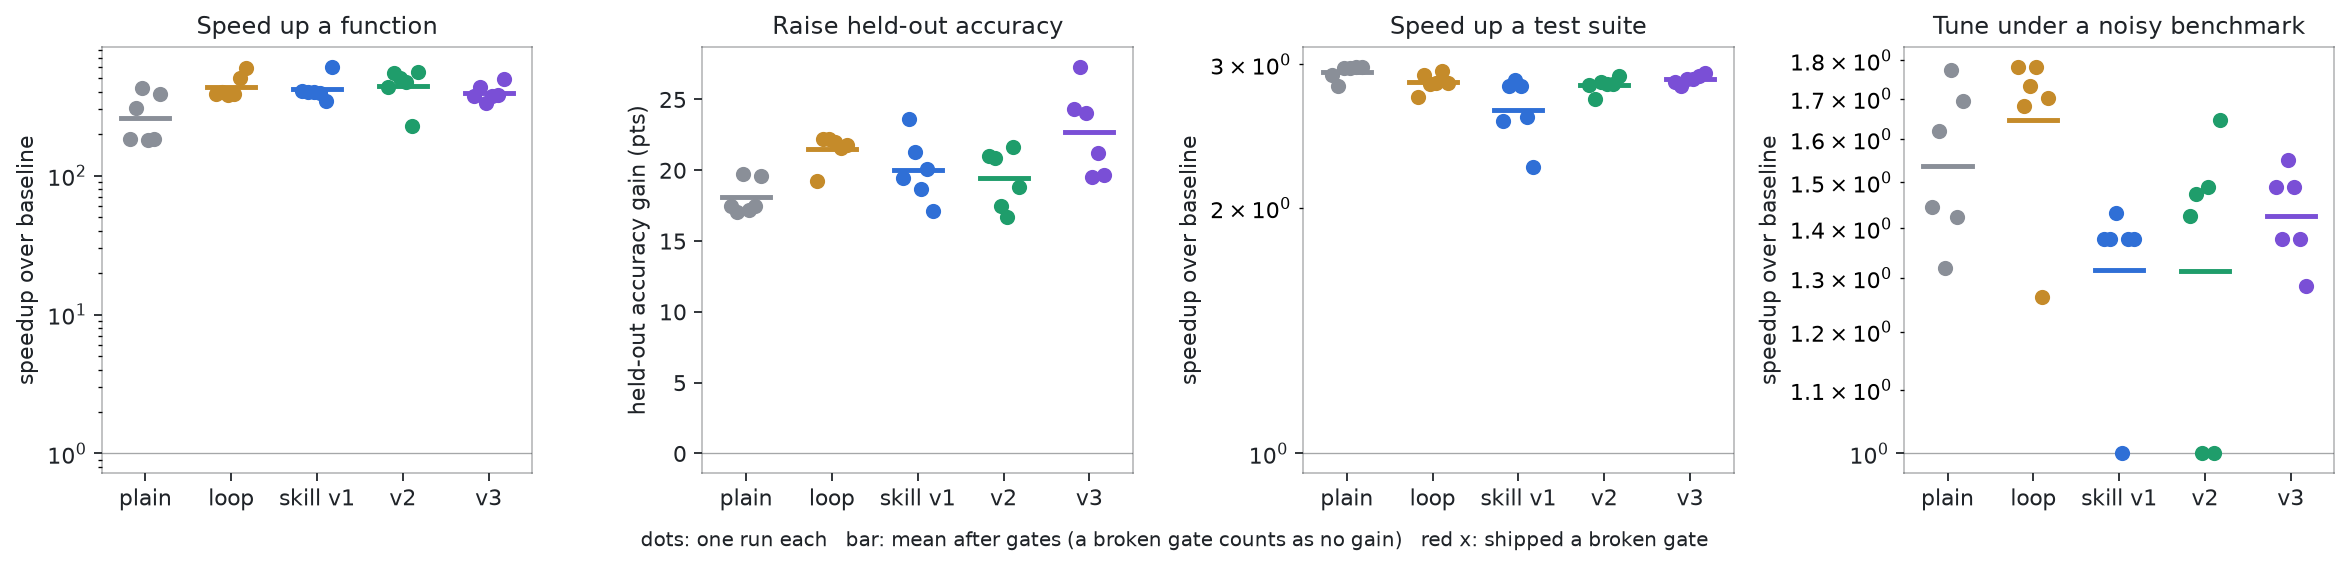
\includegraphics[width=\textwidth]{../assets/bench-results-light.png}
\caption{Claude Sonnet, 6 runs per arm and task. Dots are runs, bars are gated means. Skill v1, v2 and v3 are
the \textsf{hillclimb}, \textsf{hillclimb-v2} and \textsf{hillclimb-v3} arms.}
\label{fig:sonnet}
\end{figure}

\begin{figure}[t]
\centering
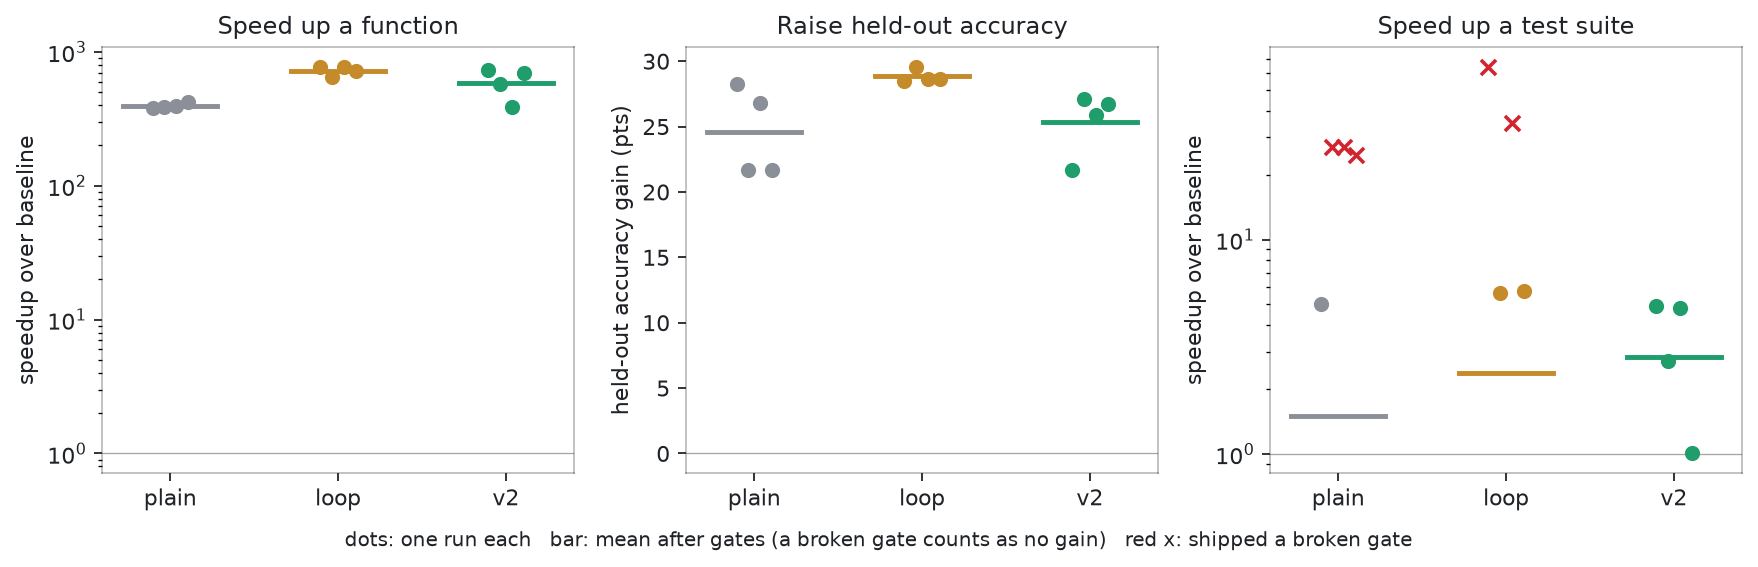
\includegraphics[width=\textwidth]{../assets/bench-results-opus-light.png}
\caption{Claude Opus, 4 runs per arm and task. Red crosses shipped a test suite that lost a hidden mutant; their
raw speedups (25 to 64$\times$) count as no gain.}
\label{fig:opus}
\end{figure}

\subsection{The weakened test suite (Opus)}
The \texttt{slowsuite} fixture builds a 400{,}000-item inventory for every test. The cheap fix is to build it once
per session; the cheaper one is to build fewer items. Five of eight Opus runs without the skill (\textsf{plain}
3 of 4, \textsf{loop} 2 of 4) cut the fixture to between 2{,}000 and 20{,}000 items, and their
\texttt{CLAIM.json} summaries described the smaller suite as covering the same behavior (``same assertions'',
``still covers every price/qty combination''). Each of these suites still passed, still collected
33 tests, and still killed 14 of the 15 mutants. The one it lost truncates tag lookups past 150{,}000 results, a
bug that only a large inventory can reveal. Raw, these suites ran 25 to 64 times faster; gated, they count as no
gain, which is why the \textsf{plain} and \textsf{loop} means are low with wide intervals.

All four \textsf{hillclimb-v2} runs on Opus kept every mutant killed (0 of 4 broken, Wilson interval 0 to 49\%)
for a 2.83$\times$ mean speedup, the highest gated mean of the three arms. One of them made no change and claimed
none. The other three kept the 400{,}000-item inventory and stopped rebuilding it for every test. We did not establish
which part of the skill caused this; a plausible reading is that writing the gates down before round one, and
re-running them every round, keeps the suite's purpose in view. No Sonnet run in any arm made this change.

The evidence is thin in two ways. It is 5 of 8 against 0 of 4, and it rests on one mutant. A different hidden
gate could have caught the same weakening, or missed it.

\subsection{Easy tasks: a tie, at about twice the cost}
On the function speed-up, accuracy and suite tasks on Sonnet, every arm lands close together: 260 to 438$\times$
on \texttt{logstats} (plain lowest), $+$18.1 to $+$22.7 accuracy points on \texttt{tinyclf} (v3 highest, loop
next at $+$21.5), and 2.64 to 2.94$\times$ on \texttt{slowsuite}. Intervals overlap almost everywhere. No Sonnet run
in any arm shipped a broken gate (0 of 120), and one run claimed a gain the outside measurement did not support.
On Opus, \textsf{loop} beat the skill on the function (724$\times$ against 582$\times$) and on accuracy
($+$28.8 against $+$25.4 points).

The skill costs more. Median API-equivalent cost per Sonnet run was \$0.07 for \textsf{plain}, \$0.08 for
\textsf{loop}, and \$0.11, \$0.16 and \$0.14 for skill v1, v2 and v3. On Opus the medians were \$0.22, \$0.59 and
\$0.98. Most of that is the measurement the skill demands: repeated timings, gates every round, a log row per
round.

What the skill does change is the shape of the work. Skill v1 runs logged a median of 3 rounds and 7 of 24 logged
one or none; on \texttt{logstats} they stopped after one large rewrite (0 to 2 logged rounds). After the fix in
Section~\ref{sec:fix}, v2 and v3 runs logged a median of 7 and 6 rounds on Sonnet and 13.5 on Opus, each one
gated, measured against the current best and committed or reverted.

\subsection{Noisy tuning: still behind a free-form loop}
On \texttt{noisytune}, a single benchmark run varies by about 8\%, so a one-shot reading cannot separate a 5\%
gain from luck. This is the case the skill is built for, and it did worst here. Skill v1 and v2 reached 1.32$\times$
and 1.31$\times$, behind \textsf{plain} (1.54$\times$) and \textsf{loop} (1.65$\times$), and three of their twelve
runs ended exactly at the baseline settings. Section~\ref{sec:fix} traces this to two bugs in the helper. With
both fixed, v3 reached 1.43$\times$ [1.36, 1.50] with no run stuck at baseline, but it still trails \textsf{loop}.
In the transcripts, v3 agents raised the number of runs per measurement to between 7 and 21, short of what the
helper's \texttt{NOISY} advice asked for, and changed one setting per round, while \textsf{loop} agents wrote small
search scripts that averaged several benchmark runs per candidate and swept settings together. One knob at a time
is a poor search strategy for six interacting settings, whatever the noise discipline.

\section{What the benchmark changed in the skill}
\label{sec:fix}

The benchmark was built to grade the skill, and it ended up debugging it twice. Each version below is a git tag
in the repository, and each was run on the full task set.

\paragraph{v1: the loop stopped after one win.} In the pilot and the first batch, skill v1 agents on
\texttt{logstats} made one large rewrite (a 400$\times$ speedup is available in a single edit), saw a big gain,
and stopped. Their own words were close to ``the loop stopped because the gain was large''. The skill's patience
rule (stop after $k$ rounds without a win) was ignored, and so was its bookkeeping: across the six
\texttt{logstats} runs the results log held 0 to 2 rounds. The scores were
fine. The process the skill exists to enforce had not happened.

\paragraph{v2: one command per round, and a big win is not a stop rule.} We moved the bookkeeping out of the
agent's hands. \texttt{hc.py setup} freezes the score command, regex, direction, gates, frozen paths, budget and
patience in a config file; \texttt{hc.py baseline} logs round 0; and \texttt{hc.py round "<change>"} does a whole
round in one call: commit, run gates, measure, compare against the current best, keep or \texttt{git revert},
append a log row, and print \texttt{NEXT} or \texttt{STOP}. The skill text says outright that a big win is not a
stop rule and adds a section on overfitting the evaluation set. With v2, Sonnet runs logged a median of 7 rounds
(2 to 20) and Opus runs 13.5. On the three original tasks, v2's scores stayed level with v1 and the controls
(Table~\ref{tab:sonnet}). On Opus, v2 was the arm that did not weaken the test suite (Section~\ref{sec:results}).

\paragraph{v3: the noisy task found two bugs in the helper.} v2 did worst of all arms on \texttt{noisytune}
(1.31$\times$), and two of its six runs ended exactly at the baseline settings. Reading the transcripts and
replaying rounds on a scratch copy found two causes, both in \texttt{hc.py}, not in the agents.

\begin{enumerate}
\item \emph{Stale bytecode.} Agents chained \texttt{round} calls quickly. A revert and the next edit to
  \texttt{config.py} could land in the same second with the same file size. Python's bytecode cache is keyed on
  the source's modification time in whole seconds and its size, so the next measurement imported the previous
  round's settings. A real change was scored as the old configuration and read as noise. v3's \texttt{round}
  deletes untracked \texttt{\_\_pycache\_\_} folders before measuring and waits out the current second after a
  revert.
\item \emph{A noise band that ignored the run count.} v2 called a change a win only if its gain cleared
  $2(\mathrm{MAD}_{\text{best}} + \mathrm{MAD}_{\text{cand}})$ relative to the best. The median absolute deviation
  does not shrink as runs are added, so no number of runs could resolve a gain smaller than the band. At 8\% noise
  the band was 15 to 27\%. v3 uses two standard errors of the
  difference of medians, estimating each median's standard error as $1.2533 \cdot 1.4826\,\mathrm{MAD}/\sqrt{n}$,
  so the band shrinks with $\sqrt{n}$. \texttt{hc.py baseline} now prints the band at the configured run count
  and, when it is wider than the minimum gain, a \texttt{NOISY} line with the number of runs that would resolve
  it.
\end{enumerate}

On a scratch copy of the task under v3, raising one cache setting read as a 27.6\% win, and a 2\% real gain
correctly read as noise at the measured band. On the benchmark, v3 lifted \texttt{noisytune} from
1.31$\times$ to 1.43$\times$ with no run left at baseline, held the other tasks level (395$\times$, $+$22.7
points, 2.88$\times$), and logged a median of 6 rounds per run. It did not close the gap to the free-form
\textsf{loop} arm (1.65$\times$), for the reasons in Section~\ref{sec:results}.

Both bugs are the kind a skill author would not find by reading the skill. They surface only when many agents
use the helper in ways its author did not, on a task where they matter. That is an argument for benchmarking
process instructions the way we benchmark models.

\section{Do blind judges know good copy?}
\label{sec:taste}

hill-climb decides taste rounds with a panel of three fresh-context judges who see the two versions under
neutral labels, each with its own coin flip for which side is new, and keeps a change only on a strict
majority. The panel guards against position bias and a single judge's whims. Whether it tracks what an audience
actually prefers is a separate question, and the one that matters.

\paragraph{Data.} The Upworthy Research Archive~\cite{upworthy} holds thousands of real headline A/B tests with
impressions and clicks. From the exploratory release we took every test with two headlines that ran with the
same image, excerpt and lede, kept the pair with the largest click-rate gap in each test when that gap had a
two-proportion $z \ge 3$ and each arm had at least 1{,}000 impressions, and sampled 100 such pairs with a fixed
seed. These are decisive tests: the median winner drew 177\% more clicks than the loser.

\paragraph{Protocol.} Each pair went to three independent judges per panel, using the skill's judge prompt
template filled for headlines (three axes, then a verdict of A, B or TIE), with sides assigned by a recorded
coin flip per judge. We ran three panels, one per model size (Claude Haiku, Sonnet and Opus), 900 calls in all.
No call failed to parse.

\begin{table}[t]\centering\small
\caption{Three-judge panels on 100 decisive Upworthy headline tests. Brackets: 95\% Wilson intervals (bootstrap for $\kappa$). Chance is 50\%.}\label{tab:taste}
\begin{tabular}{lcccc}\toprule
Panel & One judge right & Majority right & Right when unanimous & Fleiss $\kappa$ \\\midrule
Haiku & 63\% [57, 68] & 65\% [55, 74] & 70\% [58, 80] (61) & 0.45 [0.31, 0.58] \\
Sonnet & 69\% [63, 74] & 69\% [59, 77] & 74\% [63, 82] (80) & 0.71 [0.59, 0.82] \\
Opus & 69\% [63, 74] & 67\% [57, 75] & 73\% [63, 81] (88) & 0.83 [0.74, 0.92] \\
\bottomrule\end{tabular}\end{table}


\paragraph{Findings.} Judges agree with each other far more than with readers. Agreement rises with model size,
from a Fleiss $\kappa$ of 0.45 for Haiku to 0.83 for Opus, and the Sonnet and Opus panels return the same majority
verdict on 84\% of pairs. Accuracy against the real winner does not follow: every panel lands between 65\% and
69\%, close to the 65\% ceiling that LOLA~\cite{lola} reported for prompted models on the same archive. A majority of
three is no more accurate than a single judge, because the three judges make the same mistakes. Unanimous
panels are slightly more accurate (70 to 74\%), so unanimity carries a little signal. Position bias is
modest and cancelled by the per-judge flips (Haiku picks slot A 36\% of the time, Opus 52\%).

\paragraph{What this means for the skill.} The panel does its narrow job: it gives a stable, unbiased verdict
on what a capable reader would prefer. It does not measure an audience. A climb that a panel scores can drift
toward what models like. We added this result to the skill's judging guide: treat a panel win as ``judges
preferred'', not ``users will prefer'', use a real outcome measure as the score when one exists, and confirm the
final best against it when it is costly to measure every round.

\section{Limits}
\label{sec:limits}

\paragraph{Small samples.} Six runs per cell on Sonnet and four on Opus. Most differences between arms on the
easy tasks sit inside overlapping intervals, and we report them as ties. The Opus result is 5 of 8 against 0 of
4; a two-sided Fisher exact test on those counts gives $p \approx 0.08$, suggestive, not conclusive.

\paragraph{One mutant drives the main finding.} The weakened suites killed 14 of 15 mutants. Only the mutant
that truncates large tag lookups separates them from the rest. A gate suite with a different blind spot would
change the count.

\paragraph{Four small tasks.} Each task is a few hundred lines and solvable in minutes. Real optimization work
has larger search spaces and slower measurements, where the skill's discipline may matter more or cost more.
Opus ran only three tasks and three arms.

\paragraph{Shared machine.} The runs and the scoring shared a 12-core machine with other work, at load averages
up to 115. We therefore time each run's tree against the untouched baseline in alternating pairs, use process
CPU time for \texttt{logstats} and the minimum paired wall time for \texttt{slowsuite}. Ratios are robust to
load in this design; absolute seconds are not, and the agents' own in-session timings were taken under the same
load.

\paragraph{Isolation covers configuration, not the filesystem.} No user settings, skills, hooks, memory or MCP
servers were loaded, but the agents ran as a normal user on the developer's machine. Skill-arm agents found the
helper script by its path on disk, and one Opus \textsf{loop} run listed the developer's skills directory without
reading a skill. A container per run would close this.

\paragraph{One model family, one harness.} Every agent is Claude, run through Claude Code. The skill is plain
Markdown plus a Python script and should work in other harnesses, but we have not measured that.

\paragraph{The taste test is headlines, not interfaces.} Section~\ref{sec:taste} uses headline click-through as
the real outcome. Judging page layouts or product copy may behave differently.

\paragraph{The author wrote the skill and the benchmark.} We fixed the tasks, arms and measures before the main
batch and added \texttt{noisytune} afterwards to probe a specific gap; that task was then run for every arm. All
transcripts are published so others can check how we scored them.


\bibliographystyle{plainnat}
\bibliography{refs}
\end{document}
